% Errors

% B0:
% r0 <- 5
% if r0 < 10 then B1 else B2
%
% B1:
% r1 <- r0
%
% B2:
% r2 <- r0 + 2
%
% B3:
% r3 <- phi r1 r2
% r4 <- r0 + r3

\begin{definition}[Single Static Assignment (SSA)]
    A program is in SSA form iff:
    \begin{itemize}
        \item Every variable is defined \textit{exactly} once;
        \item For every variable, its definition comes before its usages;
    \end{itemize}
\end{definition}

\centering
\begin{minipage}{0.48\linewidth}
\centering
\begin{tikzpicture}[
    node distance=10mm,
    every node/.style={draw, align=left, inner sep=4pt},
    >={Stealth}
]
\node (entry)   at (0, 0)       [draw, label=above:$B_0$]   {$r_0 \leftarrow 5$ \\ if $r_0 < 10$};
\node (b1)      at (-1.7, -1.4) [draw, label=above:$B_1$]   {$r_1 \leftarrow r_0 + 1$};
\node (b2)      at (1.7, -1.4)  [draw, label=above:$B_2$]   {$r_2 \leftarrow r_0 + 2$};
\node (end)     at (0, -3)      [draw, label=above:$B_3$]   {$r_3 \leftarrow \phi(r_1, r_2)$ \\ $r_4 \leftarrow r_0 + r_3$ \\ ret $r_4$};
\draw[->] (entry) -- (b1);
\draw[->] (entry) -- (b2);
\draw[->] (b1) -- (end);
\draw[->] (b2) -- (end);
\end{tikzpicture}
\end{minipage}
\hfill
\begin{minipage}{0.48\linewidth}
\centering
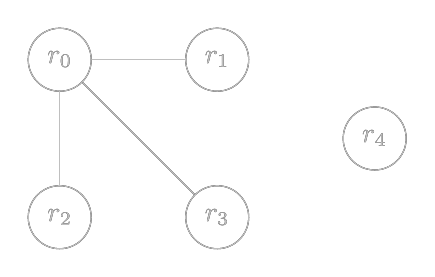
\begin{tikzpicture}[scale=1, every node/.style={circle, draw, minimum size=8mm}]
\node<1,2,3,4> (r0) at (0,0) {$r_0$};
\node<1> (r1) at (2,0) {$r_1$};
\node<1,2> (r2) at (0,-2) {$r_2$};
\node<1,2,3> (r3) at (2,-2) {$r_3$};
\node<1,2,3,4,5> (r4) at (4,-1) {$r_4$};
\node<5->[draw=lightgray, text=lightgray] (r0) at (0,0) {$r_0$};
\node<2->[draw=lightgray, text=lightgray] (r1) at (2,0) {$r_1$};
\node<3->[draw=lightgray, text=lightgray] (r2) at (0,-2) {$r_2$};
\node<4->[draw=lightgray, text=lightgray] (r3) at (2,-2) {$r_3$};
\node<6->[draw=lightgray, text=lightgray] (r4) at (4,-1) {$r_4$};

\draw<1> (r0) -- (r1);
\draw<1,2> (r0) -- (r2);
\draw<1,2,3> (r0) -- (r3);
\draw<2->[draw=lightgray] (r0) -- (r1);
\draw<3->[draw=lightgray] (r0) -- (r2);
\draw<4->[draw=lightgray] (r0) -- (r3);
\end{tikzpicture}
\end{minipage}